% Step 1 design document
% Field / format / complexity: optimizer-step schematic for MatrixPolicy. TikZ standalone, medium-density method figure.
% Five-second message: MatrixPolicy operations live on one purple matrix lane for A_l and B_l only; rational coefficients and all other tensors stay on a separate gray AdamW-only bypass lane.
% Canvas and layout: 16.7cm x 6.9cm, left-to-right optimizer step. Top band y=3.2..6.65 is the matrix lane; bottom band y=0.55..2.85 is the AdamW-only lane. Detached summaries sit above the top lane and feed only the controller.
% Modules: detached summaries, MatrixPolicy controller, RLB matrix targets, group gates, AdamW matrix branch, transient Muon substep, pair rescale, updated A_l/B_l, non-matrix tensors, AdamW-only update, updated non-matrix tensors, exclusion badge.
% Connections: purple arrows connect only top-lane matrix modules. Gray arrows connect only bottom-lane AdamW modules. Dashed gray arrows are read-only statistics, never update arrows.
% ASCII sketch:
%   [detached summaries] --read only--> [MatrixPolicy controller]
%                                      |
%   Matrix lane: [A_l,B_l] -> [group gates] -> [AdamW matrix] -> [transient Muon] -> [pair rescale] -> [updated A_l,B_l]
%
%   AdamW bypass: [rational coeffs + all other tensors] -> [AdamW only] -> [updated non-matrix tensors]     [no gates/Muon/rescale]
% Prevention notes: no vertical MatrixPolicy arrow enters the bypass lane; all connector labels are short; lane backgrounds and badges clarify exclusivity without adding update steps.
\documentclass[tikz,border=5pt]{standalone}
\usepackage{tikz}
\usepackage{amsmath,amssymb}
\usepackage[T1]{fontenc}
\usepackage{helvet}
\renewcommand{\familydefault}{\sfdefault}
\usetikzlibrary{arrows.meta,bending,calc,backgrounds}

\definecolor{mpPurple}{HTML}{6F4AA4}
\definecolor{mpPurpleFill}{HTML}{F4EFFA}
\definecolor{mpBlue}{HTML}{386B9B}
\definecolor{mpBlueFill}{HTML}{E7F0FA}
\definecolor{mpAmber}{HTML}{9B6700}
\definecolor{mpAmberFill}{HTML}{FFF2CF}
\definecolor{mpGrey}{HTML}{696969}
\definecolor{mpGreyFill}{HTML}{F3F3F3}
\definecolor{mpInk}{HTML}{202020}
\definecolor{mpRed}{HTML}{B44B4B}
\definecolor{mpRedFill}{HTML}{FBEAEA}

\pgfdeclarelayer{background}
\pgfsetlayers{background,main}

\tikzset{
  laneTitle/.style={font=\footnotesize\bfseries, anchor=west, text=mpInk},
  badge/.style={rectangle, rounded corners=2.5pt, draw=mpPurple!55, fill=white,
    line width=0.55pt, align=center, inner sep=3.2pt, font=\scriptsize},
  redBadge/.style={rectangle, rounded corners=2.5pt, draw=mpRed!75, fill=mpRedFill,
    line width=0.65pt, align=center, inner sep=3.2pt, font=\scriptsize\bfseries, text=mpRed},
  baseBox/.style={rectangle, rounded corners=3pt, line width=0.72pt, align=center,
    inner sep=4.2pt, font=\scriptsize, text=mpInk},
  matrixBox/.style={baseBox, draw=mpPurple, fill=white, minimum width=2.45cm, minimum height=1.10cm},
  opBox/.style={baseBox, draw=mpPurple, fill=white, minimum width=1.85cm, minimum height=0.90cm},
  adamBox/.style={baseBox, draw=mpBlue, fill=mpBlueFill, minimum width=1.95cm, minimum height=0.90cm},
  muonBox/.style={baseBox, draw=mpPurple, fill=mpPurpleFill, minimum width=1.70cm, minimum height=0.90cm},
  rescaleBox/.style={baseBox, draw=mpAmber, fill=mpAmberFill, minimum width=2.00cm, minimum height=0.90cm},
  outputBox/.style={baseBox, draw=mpBlue, fill=mpBlueFill, minimum width=1.85cm, minimum height=0.90cm},
  policyBox/.style={baseBox, draw=mpPurple, fill=mpPurpleFill, line width=0.9pt,
    minimum width=1.80cm, minimum height=0.66cm, font=\scriptsize\bfseries},
  statsBox/.style={baseBox, draw=mpGrey!70, fill=white, minimum width=2.60cm, minimum height=0.76cm},
  bypassBox/.style={baseBox, draw=mpGrey, fill=white, minimum height=1.04cm},
  bypassUpdate/.style={baseBox, draw=mpGrey, fill=mpGreyFill, minimum height=0.82cm, font=\scriptsize\bfseries},
  flow/.style={
    -{Stealth[length=5pt 1.5, width'=0pt 0.6, sep=0pt 0.5]},
    line width=1.0pt, shorten >=2pt, shorten <=1pt, color=mpPurple},
  flowShort/.style={
    -{Stealth[length=3pt 1.0, width'=0pt 0.5, sep=0pt 0.3]},
    line width=0.82pt, shorten >=1pt, shorten <=0pt, color=mpPurple},
  bypass/.style={
    -{Stealth[length=4pt 1.2, width'=0pt 0.6, sep=0pt 0.4]},
    line width=0.95pt, shorten >=2pt, shorten <=1pt, color=mpGrey},
  observe/.style={
    -{Stealth[length=3pt 1.0, width'=0pt 0.5]},
    densely dashed, line width=0.58pt, shorten >=1pt, shorten <=1pt, color=mpGrey!70},
  callout/.style={densely dotted, line width=0.55pt, color=mpRed!65},
  edgeLabel/.style={font=\scriptsize, inner sep=1pt, align=center},
  tinyLabel/.style={font=\tiny\bfseries, text=mpPurple},
}

\begin{document}
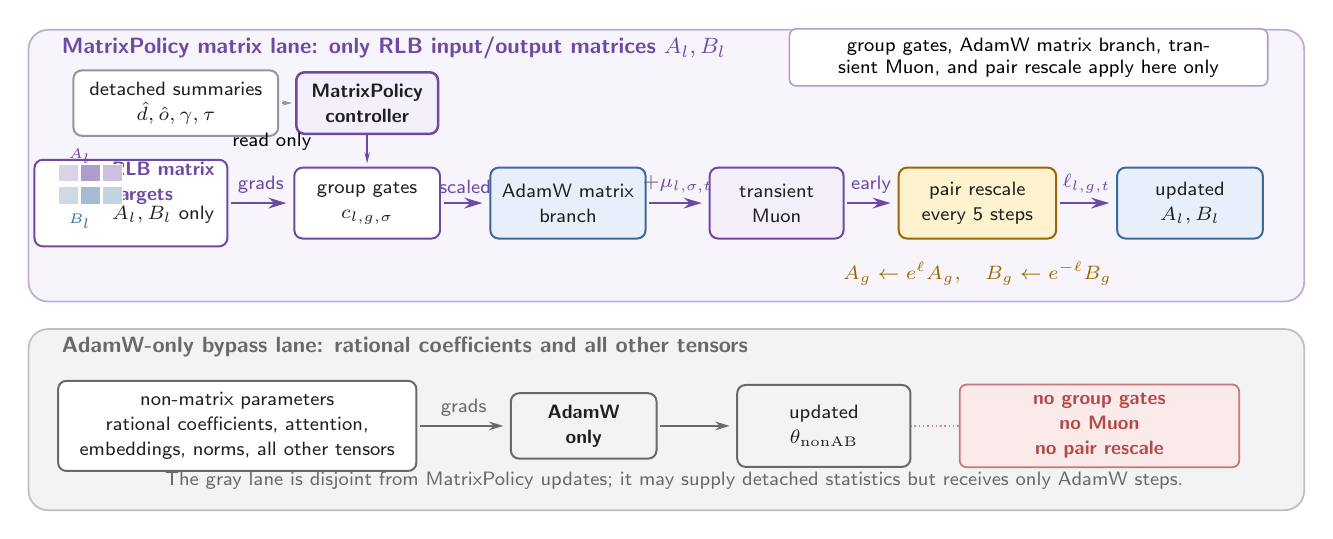
\begin{tikzpicture}[x=1cm,y=1cm]
  \begin{pgfonlayer}{background}
    \fill[mpPurpleFill!66, rounded corners=7pt] (0.25,3.20) rectangle (16.45,6.65);
    \draw[mpPurple!45, line width=0.65pt, rounded corners=7pt] (0.25,3.20) rectangle (16.45,6.65);
    \fill[mpGreyFill, rounded corners=7pt] (0.25,0.55) rectangle (16.45,2.85);
    \draw[mpGrey!42, line width=0.65pt, rounded corners=7pt] (0.25,0.55) rectangle (16.45,2.85);
  \end{pgfonlayer}

  \node[laneTitle, text=mpPurple] at (0.55,6.42)
    {MatrixPolicy matrix lane: only RLB input/output matrices $A_l,B_l$};
  \node[badge, text width=5.85cm] at (12.95,6.30)
    {group gates, AdamW matrix branch, transient Muon, and pair rescale apply here only};

  \node[laneTitle, text=mpGrey] at (0.55,2.62)
    {AdamW-only bypass lane: rational coefficients and all other tensors};

  \node[statsBox] (stats) at (2.12,5.72)
    {detached summaries\\[1pt]$\hat d,\hat o,\gamma,\tau$};
  \node[policyBox] (policy) at (4.55,5.72)
    {MatrixPolicy\\[1pt]controller};
  \draw[observe] (stats.east) -- (policy.west);
  \node[edgeLabel] at (3.34,5.23) {read only};

  \node[matrixBox] (matrices) at (1.55,4.45) {};
  \node[font=\scriptsize\bfseries, align=left, text=mpPurple] at (1.96,4.70)
    {RLB matrix\\[1pt]targets};
  \node[font=\scriptsize, align=left, text=mpInk] at (1.96,4.30)
    {$A_l,B_l$ only};

  \fill[draw=white, line width=0.25pt, fill=mpPurple!25] (0.63,4.72) rectangle ++(0.25,0.22);
  \fill[draw=white, line width=0.25pt, fill=mpPurple!55] (0.91,4.72) rectangle ++(0.25,0.22);
  \fill[draw=white, line width=0.25pt, fill=mpPurple!35] (1.19,4.72) rectangle ++(0.25,0.22);
  \fill[draw=white, line width=0.25pt, fill=mpBlue!25] (0.63,4.44) rectangle ++(0.25,0.22);
  \fill[draw=white, line width=0.25pt, fill=mpBlue!45] (0.91,4.44) rectangle ++(0.25,0.22);
  \fill[draw=white, line width=0.25pt, fill=mpBlue!30] (1.19,4.44) rectangle ++(0.25,0.22);
  \node[tinyLabel] at (0.90,5.04) {$A_l$};
  \node[tinyLabel, text=mpBlue] at (0.90,4.22) {$B_l$};

  \node[opBox] (gates) at (4.55,4.45)
    {group gates\\[1pt]$c_{l,g,\sigma}$};
  \node[adamBox] (adam) at (7.10,4.45)
    {AdamW matrix\\[1pt]branch};
  \node[muonBox] (muon) at (9.75,4.45)
    {transient\\[1pt]Muon};
  \node[rescaleBox] (rescale) at (12.30,4.45)
    {pair rescale\\[1pt]every 5 steps};
  \node[outputBox] (updatedAB) at (15.00,4.45)
    {updated\\[1pt]$A_l,B_l$};

  \draw[flowShort] (policy.south) -- (gates.north);
  \draw[flow] (matrices.east) -- node[edgeLabel, above=2pt] {grads} (gates.west);
  \draw[flow] (gates.east) -- node[edgeLabel, above=2pt] {scaled} (adam.west);
  \draw[flow] (adam.east) -- node[edgeLabel, above=2pt] {$+\mu_{l,\sigma,t}$} (muon.west);
  \draw[flow] (muon.east) -- node[edgeLabel, above=2pt] {early} (rescale.west);
  \draw[flow] (rescale.east) -- node[edgeLabel, above=2pt] {$\ell_{l,g,t}$} (updatedAB.west);

  \node[font=\scriptsize, text=mpAmber, align=center] at (12.30,3.56)
    {$A_g \leftarrow e^{\ell}A_g,\quad B_g \leftarrow e^{-\ell}B_g$};

  \node[bypassBox, minimum width=4.55cm] (other) at (2.90,1.62)
    {non-matrix parameters\\[1pt]rational coefficients, attention,\\[1pt]embeddings, norms, all other tensors};
  \node[bypassUpdate, minimum width=1.85cm] (adamOnly) at (7.30,1.62)
    {AdamW\\[1pt]only};
  \node[bypassBox, fill=mpGreyFill, minimum width=2.20cm] (updatedOther) at (10.35,1.62)
    {updated\\[1pt]$\theta_{\mathrm{nonAB}}$};
  \node[redBadge, minimum width=3.55cm] (noops) at (13.85,1.62)
    {no group gates\\[1pt]no Muon\\[1pt]no pair rescale};

  \draw[bypass] (other.east) -- node[edgeLabel, above=2pt] {grads} (adamOnly.west);
  \draw[bypass] (adamOnly.east) -- (updatedOther.west);
  \draw[callout] (noops.west) -- (updatedOther.east);

  \node[font=\scriptsize, text=mpGrey, align=center] at (8.45,0.92)
    {The gray lane is disjoint from MatrixPolicy updates; it may supply detached statistics but receives only AdamW steps.};
\end{tikzpicture}
\end{document}
